\section{Model Card: Future Statement Model}
This model is a finetuned on 2500 expressions, which contained 1250 future statements. distilbert-base-uncased serves as a base model
\\
\\
%
\textbf{Model Description}
%
\begin{itemize}
    \item Huggingface name: distilbert-base-future
    \item Creation Date: 11/08/22
    \item Version: 1.0
    \item model type: text classification
\end{itemize}%
%
\textbf{Intended Use \& Limitations}
%
\begin{itemize}
    \item The primary intended use is the classification of input into a future or non-future sentence/statement.
    \item The model is primarily intended to be used by researchers to filter or label a large number of sentences according to the grammatical tense of the input.
\end{itemize}%
%
\textbf{Hyperparameters}
\\
\\
The following hyperparameters were used during training
\begin{itemize}
    \item optimizer:
    name: Adam, learning\_rate: 5e-05, decay: 0.0, beta\_1: 0.9, beta\_2: 0.999, epsilon: 1e-07, amsgrad: False
    \item training\_precision: float32
\end{itemize}%
\label{sec:appendix}
%
\textbf{Training Results}
\\
For finetuning, we have 80\% of of records from our self-annotated future-tatements dataset. This corresponds to 2000 records.
The remaining 500 will be used to test the final distilbert-base-future model
\\
%%%%%%%%%%%%%%%%%%%%%%%%%%%%%%%%%%%%%%%%%%%%%%%%%%%%%%%%%%%%%%%%%%%%%%%%%%%%%%%%%%%%%%%%%%%%%%%%%%%%%%%%%%%%%%%%%%%%%%%%%%%%%%%%%%%%%%%%%%%%%%%%%%%%%%
%%%%%%%%%%%%%%%%%%%%%%%%%%%%%%%%%%%%%%%%%%%%%%%%%%%%%%%%%%%%%%%%%%%%%%%%%%%%%%%%%%%%%%%%%%%%%%%%%%%%%%%%%%%%%%%%%%%%%%%%%%%%%%%%%%%%%%%%%%%%%%%%%%%%%%
\begin{table}[ht]
    \scriptsize
    \setlength\tabcolsep{10pt} % let LaTeX compute intercolumn whitespace
    \footnotesize\centering
    \begin{tabular}{ccccc}
        \toprule
        \textbf{Epoch} & \textbf{Train Loss} & \textbf{Train Accuracy} & \textbf{Val. Loss} & \textbf{Val. Accuracy} \\
        \midrule
        0 & 0.3816 & 0.8594 & 0.1547 & 0.9475 \\
        1 & 0.1142 & 0.9613 & 0.1272 & 0.9625 \\
        \bottomrule
    \end{tabular}
    \caption{\label{future-model-train}
    Training Results
    }
\end{table}
%%%%%%%%%%%%%%%%%%%%%%%%%%%%%%%%%%%%%%%%%%%%%%%%%%%%%%%%%%%%%%%%%%%%%%%%%%%%%%%%%%%%%%%%%%%%%%%%%%%%%%%%%%%%%%%%%%%%%%%%%%%%%%%%%%%%%%%%%%%%%%%%%%%%%%
%%%%%%%%%%%%%%%%%%%%%%%%%%%%%%%%%%%%%%%%%%%%%%%%%%%%%%%%%%%%%%%%%%%%%%%%%%%%%%%%%%%%%%%%%%%%%%%%%%%%%%%%%%%%%%%%%%%%%%%%%%%%%%%%%%%%%%%%%%%%%%%%%%%%%%
%
%
\\
\textbf{Framework versions}
\begin{itemize}
    \item Transformers 4.18.0
    \item Tensorflow 2.8.0
    \item Tokenizers 0.12.1
\end{itemize}%
%
\pagebreak
\textbf{Test Set Results}
\begin{figure}[h]
    \centering
    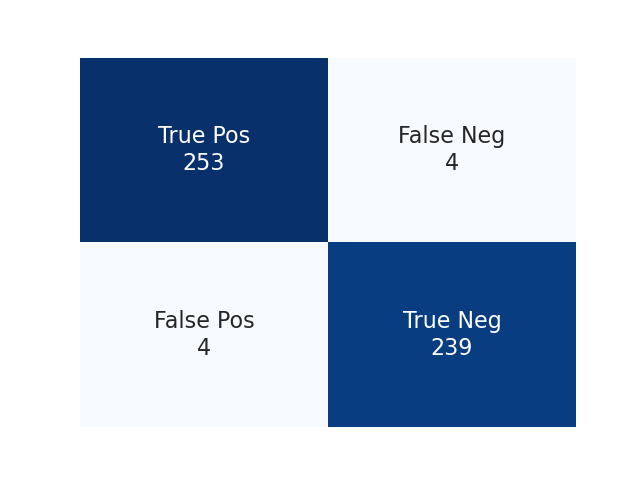
\includegraphics[width=0.5\textwidth]{cm}
    \caption{
        Confusion matrix after applying the test set with the resulting accuracy of 93,8\%.
    }
    \label{fig:cm}
\end{figure}
